\subsubsection{MHD: Orszag-Tang Vortex}
\label{sec.tests.mhd}
Figure~\ref{fig.orszag} shows the Orszag-Tang vortex problem, a
standard magnetohydrodynamic test problem \citep{Orszag79}.  The left panel shows
the result using \enzo's constrained transport MHD method, while the right panel shows the result using
\enzo's implementation of Dedner MHD.
The Orszag-Tang vortex test shows that significant small scale structure can be generated in MHD
from large scale initial perturbations, and is used to compare the
effective resolution of different MHD schemes.  The test begins with uniform
density, $\rho_0=25/36 \pi$ and pressure, $P_0=5/12 \pi$ (as with
other tests in this section, in the absence of gravity or chemistry we use
arbitrary units).  There is a
single rotational mode in the velocity, and two in the magnetic field:
${\bf v}_0 $ = (-sin(2$\pi$ y) $ \hat{x}$ , sin(2$\pi$ x) $\hat{y}$),
${\bf B}_0$ = (-sin(2 $\pi$ y) $ \hat{x},$ sin( 4 $\pi$ x )$\hat{y}$).
The simulation is evolved to $t=0.48$ (in arbitrary units).  One can see that the structures
are accurately represented as compared to, for instance,
\citet{Toth00}, and that the resolution of shocks is comparable in
both methods.

\begin{figure}
\begin{center}
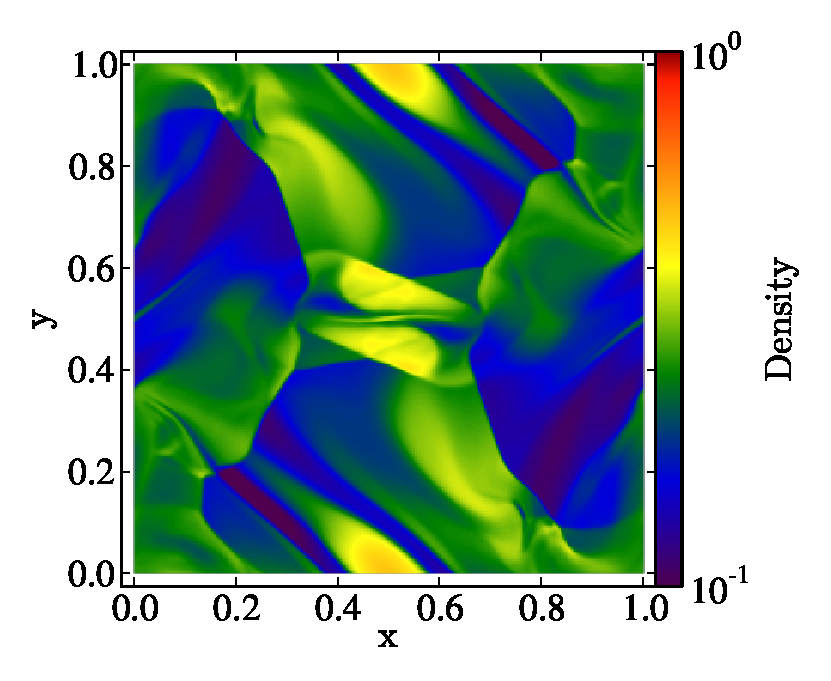
\includegraphics[width=0.4\textwidth]{figures/MHDCT_OrszagTang_Density.eps}
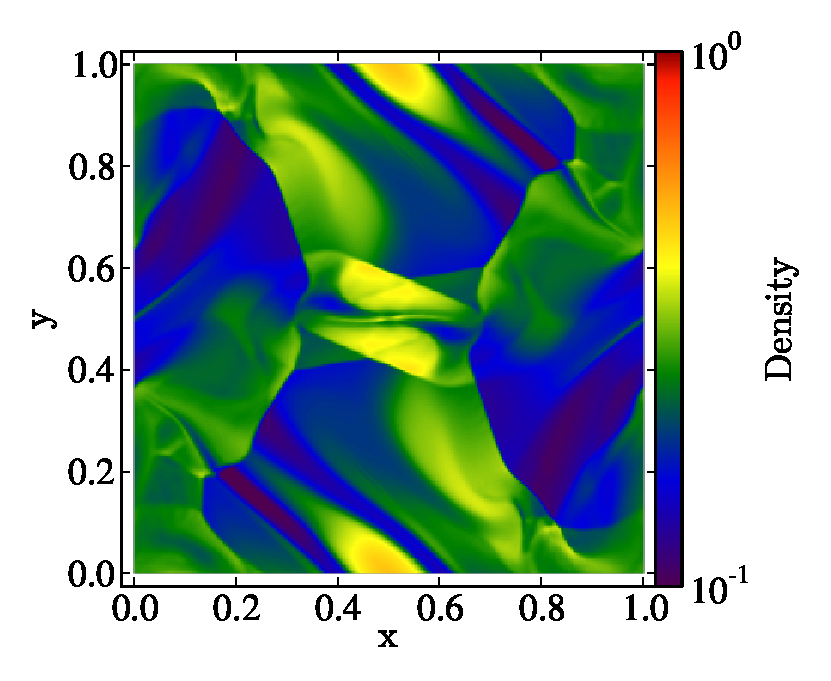
\includegraphics[width=0.4\textwidth]{figures/MHDDedner_OrszagTang_Density.eps}
\caption{Density field from the Orszag-Tang vortex test, at $t=0.48$.
Left: solution using constrained transport MHD.  Right: solution using
Dedner MHD. The initial conditions are uniform density, with a single
rotating velocity structure and two circular magnetic structures.
These initial conditions generate significant small-scale structure in
both the CT and Dedner schemes, which have approximately equal
effective resolution.}
\label{fig.orszag}
\end{center}
\end{figure}
